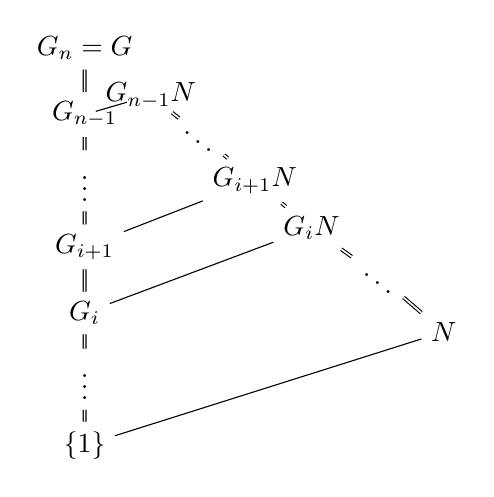
\begin{tikzpicture}[scale=1.2]
  % Nodes
  \node (Gn) at (-1,2.1) {$G_n=G$};
  \node (Gn-1) at (-1,1.4) {$G_{n-1}$};
  \node (p1) at (-1,0.7) {$\vdots$};
  \node (Gi+1) at (-1,0) {$G_{i+1}$};
  \node (Gi) at (-1,-0.7) {$G_i$};
  \node (p2) at (-1,-1.4) {$\vdots$};
  \node (1) at (-1,-2.1) {$\{1\}$};
  \node (Gn-1N) at (-0.3,1.6) {$G_{n-1}N$};
  \node (p3) at (0.2,1.2) {$\ddots $};
  \node (Gi+1N) at (0.8,0.7) {$G_{i+1}N$};
  \node (GiN) at (1.4,0.2) {$G_iN$};
  \node (p4) at (2.1,-0.3) {$\ddots$};
  \node (N) at (2.8,-0.9) {$N$};

  % Lineas nodos
  \draw[double] (Gn) -- (Gn-1);
  \draw[double] (Gn-1) -- (p1);
  \draw[double] (p1) -- (Gi+1);
  \draw[double] (Gi+1) -- (Gi);
  \draw[double] (Gi) -- (p2);
  \draw[double] (p2) -- (1);
  \draw (Gn-1) -- (Gn-1N);
  \draw (Gi+1) -- (Gi+1N);
  \draw (Gi) -- (GiN);
  \draw (1) -- (N);
  \draw[double] (Gn-1N) -- (p3);
  \draw[double] (p3) -- (Gi+1N);
  \draw[double] (Gi+1N) -- (GiN);
  \draw[double] (GiN) -- (p4);
  \draw[double] (p4) -- (N);
\end{tikzpicture}
